\documentclass[simplex.tex]{subfiles}
% NO NEED TO INPUT PREAMBLES HERE
% packages are inherited; you can compile this on its own
\begin{document}
\subsection{knor: K-means NUMA Optimized Routines}

%% Jan

As part of our commitment to readily available tools
we migrated \textsf{knor} to the FlashX organization
\href{https://github.com/flashxio}{https://github.com/flashxio} to increase
visibility. Furthermore, we extended the capability of \textsf{knor} by
providing the option of using \textsf{knor} as an initialization tool
for other clustering algorithms. The intention is to allow users to
seamlessly add \textsf{knor} to their workflow.
We pushed a new release named \textit{african jallof} to
provide this capability: \\
\href{https://github.com/flashxio/knor/releases}
{https://github.com/flashxio/knor/releases}.

We benchmarked our Semi-external memory routine, \textsf{knors} in the cloud
using Amazon EC2 using a single 32 core i3.16xlarge machine with 8 SSDs on Amazon EC2 compared
to \textsf{knord}, MLlib and an optimized MPI routine running in a cluster.
We run \textsf{knors} with 48 threads, with extra parallelism coming
from symmetric multiprocessing. We show comparable to in-memory
performance and outperform MLlib with much less hardware resources.
We added these results the paper which shall be published in HPDC '17.

\begin{table}[!htb]
    \caption{The datasets under evaluation in this study. \textit{Friendster}
    %\citereferences{friendster}
        is a social network. We obtain the graph containing friend relationships and
compute Eigenvalues and Eigenvectors.}
\vspace{-10pt}
\begin{center}
\footnotesize
\begin{tabular}{|c|c|c|c|}
\hline
\textbf{Data Matrix} & $n$ & $d$ & \textbf{Size}\\
\hline
Friendster-8 eigenvectors & $66$M &
  $8$ & $4$GB\\
\hline
Friendster-32 eigenvectors & $66$M &
  $32$ & $16$GB\\
\hline
Rand-Multivariate (RM-856M)& $856$M & 16 & $103$GB\\
\hline
Rand-Multivariate (RM-1B)& $1.1$B & 32 & $251$GB\\
\hline
\end{tabular}
\normalsize
\end{center}
\label{tbl:matrices}
\end{table}

\begin{figure}[!h]
\begin{cframed}
    \centering
    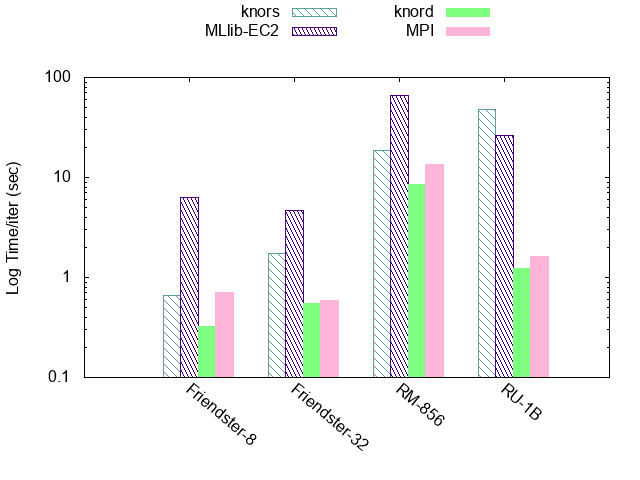
\includegraphics[width=.5\textwidth]{../../figs/perf.iter.sem-ec2.png}
\caption{Performance comparison of \textsf{knors} to distributed packages.
\textsf{knors} uses one i3.16xlarge machine with 32 physical cores.
\textsf{knord}, MLlib-EC2 and MPI use 3 c4.8xlarge with a total of 48 physical
cores for all datasets other than RU-1B where they use 8 c4.8xlarge with a
total of 128 physical cores.}
\label{fig:sem-ec2}

\end{cframed}
\end{figure}
\clearpage

\end{document}
